\documentclass[10pt]{article}

\usepackage[margin=0.82in]{geometry}
\usepackage[T1]{fontenc}
\usepackage[utf8]{inputenc}
\usepackage{lmodern}
\usepackage{microtype}
\usepackage{amsmath,amssymb}
\usepackage{booktabs}
\usepackage{tabularx}
\usepackage{array}
\usepackage{graphicx}
\usepackage{xcolor}
\usepackage{caption}
\usepackage{float}
\usepackage{enumitem}
\usepackage{listings}
\usepackage[hidelinks]{hyperref}

\graphicspath{{../../images/}}
\captionsetup{font=small,labelfont=bf}
\setlength{\parindent}{0pt}
\setlength{\parskip}{0.38em}
\renewcommand{\arraystretch}{1.12}
\newcolumntype{Y}{>{\raggedright\arraybackslash}X}

\lstset{
  basicstyle=\ttfamily\footnotesize,
  columns=fullflexible,
  frame=single,
  rulecolor=\color{black!35},
  backgroundcolor=\color{black!03},
  xleftmargin=0.3em,
  xrightmargin=0.3em,
  aboveskip=0.55em,
  belowskip=0.55em,
  showstringspaces=false
}

% Replace this box with the requested experimental figure before submission.
\newcommand{\figureplaceholder}[3]{%
  \begin{figure}[H]
    \centering
    \fbox{\parbox[c][#1][c]{0.91\linewidth}{\small\raggedright
      \textbf{Figure to insert.} #2}}
    \caption{#3}
  \end{figure}%
}

\title{\textbf{Scalable PDDL Planning for Urban Routing under Dynamic Traffic}\\
\large Routly Planner: compiled traversal actions, hybrid congestion, and macro-road abstraction}
\author{Author Name \and Collaborator Name}
\date{July 2026}

\begin{document}
\maketitle

\begin{abstract}
Routly Planner converts an OpenStreetMap road network into a PDDL/PDDL+
planning problem, computes a route with ENHSP, and validates the route in SUMO.
The challenge is to preserve routing constraints such as congestion, fuel, road
closures, and time while preventing the grounded planning problem from growing
with every road, location, and time window. This report presents the modelling
choices and implementation strategy adopted for this purpose. We distinguish a
PDDL+ process model, retained for controller-based replanning, from a lighter
compiled-duration model that represents a road crossing as a direct numeric
transition. The latter is combined with globally indexed congestion windows,
hybrid selection of time-varying roads, singleton-typed compiled actions, and
an optional macro-road abstraction. The report defines a reproducible
experimental protocol and separates measured evidence from results that must be
collected from ENHSP logs before final submission.
\end{abstract}

\noindent\textbf{Keywords:} automated planning; PDDL+; time-dependent routing;
traffic congestion; grounding; road-network abstraction.

\section{Problem Description}
Routly receives a directed road graph $G=(L,R)$, a vehicle $v$, a start location,
and a goal location. The planner must select a feasible route that minimises a
numeric plan metric while respecting road availability, optional fuel limits,
and traffic-dependent travel costs. SUMO remains the physical simulator; PDDL
is the decision layer that chooses the route. This distinction follows the
time-dependent routing perspective in \cite{baum2015}.

In the static congestion model, each road $r$ receives one factor $c_r$ computed
from background traffic and keeps it for the complete plan. The resulting cost
is fixed. Dynamic congestion instead associates a road with a sequence of
window factors $c_{r,w}$, where $w$ identifies a global time interval. This is
more faithful to time-dependent routing, but it raises the symbolic cost of the
planning problem.

The central scalability issue is not traffic simulation itself, but the
parameterisation exposed to the planner. A generic dynamic traversal schema has
parameters for a vehicle, road, origin, destination, and time window. A loose
type-compatible upper bound is therefore
\[
  N_{\mathrm{generic}} = O\!\left(|V|\,|R|\,|L|^2\,|W|\right).
\]
For example, $677$ roads, $384$ locations, one vehicle, and $14$ windows yield
approximately $1.40\times10^9$ type-compatible tuples before topological
preconditions such as \texttt{connects} remove invalid combinations. In the
static case the $|W|$ factor disappears, but the road--location product remains
large. Thus dynamic congestion magnifies an existing grounding problem rather
than creating it from nothing.

\section{Modelling}
\subsection{Traversal semantics}
The original PDDL+ model represents a crossing with a start action, a continuous
process, and an arrival event \cite{fox2006,coles2012}. It is useful when the vehicle must be observable
inside a road. However, start-to-goal route selection does not require that
intermediate state, so the compiled-duration model replaces it with one numeric
transition, in the spirit of temporal-numeric compilation approaches
\cite{micheli2026}. This reduces processes, arrival events, and continuous numeric
evolution while preserving the route-level cost.

\begin{table}[t]
\centering
\caption{Planner configurations and their role in Routly.}
\label{tab:planner-configurations}
\small
\begin{tabularx}{\linewidth}{@{}l l l Y@{}}
\toprule
Traversal model & State & Actions & Role and status \\
\midrule
\texttt{process} & node-based & parameterized & Implemented PDDL+ model for controller-based partial plans. \\
\texttt{compiled\_duration} & node-based & parameterized & Generic grounding baseline. \\
\texttt{compiled\_duration} & node-based & compiled & Implemented planner-side scalability configuration. \\
\texttt{compiled\_duration} & line graph & parameterized or compiled & Implemented experimental road-state formulation. \\
\bottomrule
\end{tabularx}
\end{table}

The generic compiled-duration action uses symbolic road and location variables:
\begin{lstlisting}
(:action traverse-road
  :parameters (?v - vehicle ?r - road ?from ?to - location)
  :precondition (and (at ?v ?from) (connects ?r ?from ?to)
                     (road-open ?r))
  :effect (and (not (at ?v ?from)) (at ?v ?to)
               (increase (travel-time ?v) (travel-duration ?r))))
\end{lstlisting}

The current scalable configuration compiles one action schema for each valid
road transition. Singleton types bind the road, endpoints, and, for a dynamic
road, the selected window. The PDDL syntax still contains variables, but each
associated type has exactly one admissible object; the planner does not need to
construct unrelated road--location combinations.
\begin{lstlisting}
(:action traverse-road-dynamic-road_001-tw_00030
  :parameters (?v - vehicle ?r - road_type_road_001
               ?from - loc_type_loc_a ?to - loc_type_loc_b
               ?w - window_type_tw_00030)
  :precondition (and (at ?v ?from) (connects ?r ?from ?to)
                     (road-open ?r) (dynamic-road ?r)
                     (current-window ?w))
  :effect (and (not (at ?v ?from)) (at ?v ?to)
               (increase (travel-time ?v)
                         (travel-duration-window ?r ?w))
               (increase (sim-time)
                         (travel-duration-window ?r ?w))))
\end{lstlisting}

With $S$ static roads, $D$ dynamic roads, and $|W|$ global windows, this
generation strategy emits $S+D|W|$ valid traversal schemas rather than exposing
a Cartesian product to the grounder. The domain file grows, but its actions are
already filtered by the Python-side road topology.

The line-graph formulation changes the planning state from a location to the
next road to be traversed. Scenario selection remains node-based: the PDDL
generation step computes the shortest path between the selected start and goal
locations and uses the first road as the initial \texttt{ready-road} and the
last road as the unique \texttt{goal-road}. Traversal actions then move from one
road to the next through \texttt{road-next}; a \texttt{finish-road} action marks
the goal as reached. This is an explicit modelling assumption: the start and
goal locations selected by the scenario are converted to roads by running a
deterministic Dijkstra search on the directed planning graph, using road length
as edge weight and road identifiers as a stable tie-breaker. Therefore line
graph experiments do not choose arbitrary start or goal roads; they use the
first and last road of the shortest start-node--goal-node route.

\subsection{Global-window hybrid congestion}
The dynamic model uses one global predicate \texttt{(current-window ?w)}. Its
successor relation and an \texttt{advance-window} event move the global state;
a dynamic traversal reads \texttt{travel-duration-window} for the window active
when the vehicle enters the road. Static roads retain one
\texttt{travel-duration}. This avoids separate temporal updates for every
road/window pair.

Hybrid congestion selects a road as dynamic only when its temporal range is
meaningful:
\[
  \max_w c_{r,w} - \min_w c_{r,w} \geq \theta,
\]
where the current empirical configuration sets $\theta=0.10$. Roads below the
threshold remain static. If no road passes the test, the run is valid and
behaves as static congestion; it does not fail. This criterion replaced earlier
top-traffic, corridor, and candidate-path heuristics because those rules could
mark roads dynamic even when their cost was effectively time-invariant.

\section{Implementation}
The implementation is organised around three independent configuration axes:
traversal semantics, state representation, and action generation. The relevant
YAML configuration for the scalable planner is shown below. The process model
is intentionally constrained to node-based, parameterized actions, whereas the
compiled-duration model supports node-based and line-graph state
representations with parameterized or compiled action generation.

\begin{lstlisting}
planner:
  traversal_model: "compiled_duration"
  state_representation: "node_based"
  action_generation: "compiled"

features:
  congestion:
    enabled: true
    mode: "pddl"
    type: "hybrid"
    dynamic:
      window_seconds: 30
      hybrid:
        min_temporal_variation: 0.10
  road_abstraction:
    enabled: true
\end{lstlisting}

Macro-road abstraction is an optional preprocessing step. It merges linear
chains whose intermediate nodes do not represent decisions. Start and goal
locations, fuel stations, traffic lights, and branching intersections remain
protected. The aggregate preserves length and uses a length-weighted harmonic
speed so that its travel time equals the sum of the underlying micro-road
times. Each macro-road also stores its expansion to physical roads, allowing
SUMO, background traffic, and LLM events to remain grounded in the original
network.

\begin{figure}[H]
  \centering
  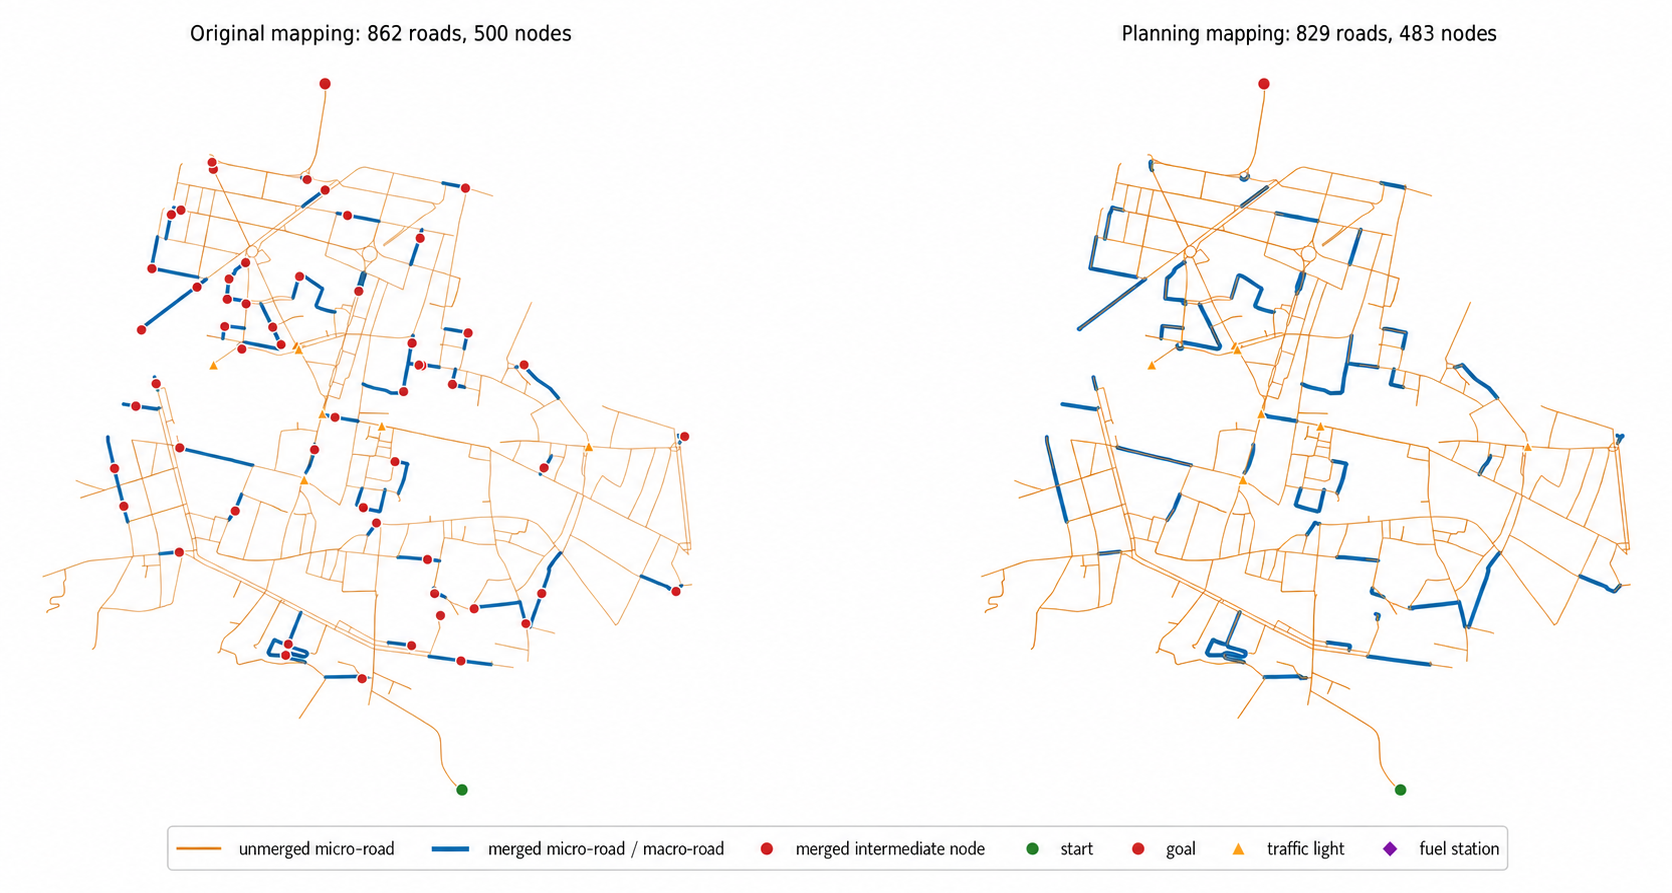
\includegraphics[width=0.93\linewidth]{macro_roads_comparison.png}
  \caption{Macro-road abstraction in the latest 500-node Bologna experiment.
  The planning graph changes from 702 roads and 393 nodes to 676 roads and 383
  nodes; 90 micro-roads are grouped into 41 macro-roads.}
  \label{fig:macro-roads}
\end{figure}

\begin{table}[H]
\centering
\caption{Measured topology reduction in the macro-road experiment.}
\label{tab:macro-measurement}
\small
\begin{tabular}{@{}lrrr@{}}
\toprule
Planning representation & Roads & Nodes & Change \\
\midrule
Original mapping & 702 & 393 & -- \\
Macro-road mapping & 676 & 383 & $-26$ roads, $-10$ nodes \\
\bottomrule
\end{tabular}
\end{table}

The implementation deliberately separates two scalability paths. Planner-side
optimisation uses \texttt{compiled\_duration} and compiled actions. Controller-side
optimisation retains the PDDL+ process model and joins partial plans outside the
planner. Fuel and congestion replanning controllers are mutually exclusive, so
their assumptions cannot be mixed in one run.

\section{Results and Experimental Protocol}
All comparisons should use the same map seed, start/goal pair, background
traffic, Java heap, ENHSP version, and SUMO scenario. The required measurements
are: PDDL object count, domain/problem size, generated action schemas, grounding
time, search time, expanded nodes, peak memory when available, plan metric, and
SUMO route validity. This protocol tests whether a smaller symbolic model also
improves search without degrading the final route.

Table~\ref{tab:results-template} is intentionally a results template rather
than a source of fabricated performance claims. Populate it from the saved
\texttt{runs/basic} ENHSP logs for the same scenario. The macro-road counts in
Table~\ref{tab:macro-measurement} are the currently verified structural result;
timing values must be reported only after the corresponding run is reproduced.

\begin{table}[H]
\centering
\caption{Results table to complete from reproducible ENHSP runs.}
\label{tab:results-template}
\scriptsize
\begin{tabularx}{\linewidth}{@{}Y l r r r r Y@{}}
\toprule
Configuration & Map & Action schemas & Grounding (s) & Search (s) & Expanded nodes & Outcome \\
\midrule
Process, parameterized & 500 nodes & [fill] & [fill] & [fill] & [fill] & PDDL+ controller baseline \\
Compiled duration, parameterized & 500 nodes & [fill] & [fill] & [fill] & [fill] & Generic grounding baseline \\
Compiled duration, compiled & 500 nodes & [fill] & [fill] & [fill] & [fill] & Singleton-typed valid actions \\
Compiled + macro roads + hybrid & 500 nodes & [fill] & [fill] & [fill] & [fill] & Full scalable configuration \\
\bottomrule
\end{tabularx}
\end{table}

\figureplaceholder{0.21\textheight}{Insert a single, no-fuel route comparison
from the same 500-node run: the original and replanned routes plus LLM event
markers. The recommended source is \texttt{images/no\_fuel\_event\_map.png};
retain the legend so that route changes are attributable to closures and
slowdowns rather than fuel constraints.}{Route-level validation after LLM event
injection. The figure should contrast the original route, the replanned route,
and the roads or intersections affected by the event.}

% Optional additional evidence, only if the final paper remains within six pages:
% place no_fuel_congestion_pre.png and no_fuel_congestion_post.png side by side
% to show how the congestion field changes without fuel as a confounding factor.

\section{Conclusions}
The report identifies modelling granularity as the main source of poor
scalability in the original road-routing encoding. Static and dynamic congestion
share the same basic grounding risk; time windows multiply it. The implemented
response is to use compiled-duration traversal when mid-road vehicle state is
not needed, expose only valid road/window actions through singleton types, and
preserve temporal realism with global-window hybrid congestion. Macro-road
abstraction further reduces the planning graph while keeping a reversible mapping
to SUMO roads.

The line-graph representation remains a principled future comparison. It can
reduce the parameter space of a generic model by making roads rather than nodes
the vehicle state, but it is not currently implemented and should not be
presented as an experimental result. The final evaluation must complete
Table~\ref{tab:results-template} and verify that every reported PDDL route
expands to a valid SUMO route. This provides a focused contribution: a
reproducible study of how domain-specific compilation and abstraction affect
time-dependent urban route planning.

\begin{thebibliography}{9}

\bibitem{fox2006}
M. Fox and D. Long.
\newblock Modelling Mixed Discrete-Continuous Domains for Planning.
\newblock \emph{Journal of Artificial Intelligence Research}, 27:235--297,
2006. \url{https://arxiv.org/abs/1110.2200}

\bibitem{coles2012}
A. Coles et al.
\newblock COLIN: Planning with Continuous Linear Numeric Change.
\newblock \emph{Journal of Artificial Intelligence Research}, 44:1--96,
2012. \url{https://arxiv.org/abs/1401.5857}

\bibitem{baum2015}
M. Baum, J. Dibbelt, T. Pajor, and D. Wagner.
\newblock Dynamic Time-Dependent Route Planning in Road Networks with User
Preferences. 2015. \url{https://arxiv.org/abs/1512.09132}

\bibitem{piotrowski2023}
W. Piotrowski et al.
\newblock Heuristic Search for Physics-Based Problems: Angry Birds in PDDL+.
2023. \url{https://arxiv.org/abs/2303.16967}

\bibitem{piotrowski2024}
W. Piotrowski and M. A. Perez.
\newblock Real-World Planning with PDDL+ and Beyond.
2024. \url{https://arxiv.org/abs/2402.11901}

\bibitem{micheli2026}
A. Micheli, E. Scala, and A. Valentini.
\newblock Compiling Temporal Numeric Planning into Discrete PDDL+.
2026. \url{https://arxiv.org/abs/2603.12188}

\bibitem{routlycode}
G. Rudi et al.
\newblock Routly Planner source code and reproducible experiment artefacts.
\url{https://github.com/GiuseppeRudi/routly-planner}

\end{thebibliography}

\end{document}
